\documentclass[aspectratio=169,9pt]{beamer}
\usetheme[progressbar=frametitle,numbering=fraction]{metropolis}
\usepackage[utf8]{inputenc}
\usepackage[T1]{fontenc}
\usepackage{amsmath,amssymb,bm}
\usepackage{graphicx}
\usepackage{booktabs}
\usepackage{tabularx}
\usepackage{siunitx}
\usepackage{tikz}
\usetikzlibrary{arrows.meta,calc,patterns,decorations.pathmorphing}
\sisetup{detect-all}
\definecolor{cBlue}{HTML}{2A6FBB}
\definecolor{cRed}{HTML}{D62839}
\definecolor{cGreen}{HTML}{2A9D55}
\definecolor{cOrange}{HTML}{E07B39}
\definecolor{cGrey}{HTML}{6B7280}
\newcommand{\um}{\,\si{\micro\metre}}
\DeclareMathOperator*{\med}{med}

\title{Viscoelastic Ting fit of AFM force curves}
\subtitle{From the raw signal to $E_1$, $\alpha$ and $E(t)$ maps: every step, the math, and what each parameter does}
\date{Worked example: data\_213626 (Ciona embryo), 37 $\times$ 75 curves, colloidal probe $R=\SI{3}{\micro\metre}$}
\author{}

\begin{document}
\maketitle

\begin{frame}{Contents}
\begin{columns}[T]
\begin{column}{0.48\textwidth}
\begin{enumerate}
\item The model in one slide
\item Raw signal $\to$ force: calibration, drag, baseline, averaging
\item Tip position, contact point, indentation
\item Elastic contact law (sphere, paraboloid, cone)
\item Power-law relaxation $E(t)$
\item Loading (Lee--Radok) and unloading (Ting)
\end{enumerate}
\end{column}
\begin{column}{0.48\textwidth}
\begin{enumerate}\setcounter{enumi}{6}
\item Discretisation and the fit
\item Worked example, and what each parameter does
\item Are $E_1$ and $\alpha$ separable?
\item Surface-slope correction
\item Validity checks, outputs, maps
\item All parameters, sensitivities, limits
\end{enumerate}
\end{column}
\end{columns}
\end{frame}

\begin{frame}{The model in one slide}
\small
A sphere is pushed into the sample and pulled back. The sample is a viscoelastic half-space whose relaxation modulus follows a power law:
\[E(t)=E_1\Bigl(\frac{t}{t_0}\Bigr)^{-\alpha},\qquad t_0=\SI{1}{\second}\]
\textbf{Approach} (contact area grows), Lee--Radok:
\[F(t)=\frac{1}{1-\nu^2}\int_0^{t}E(t-\tau)\,\frac{d\varphi(\delta(\tau))}{d\tau}\,d\tau\]
\textbf{Retract} (contact area shrinks), Ting:
\[F(t)=\frac{1}{1-\nu^2}\int_0^{t_1(t)}E(t-\tau)\,\frac{d\varphi(\delta(\tau))}{d\tau}\,d\tau,\qquad \int_{t_1(t)}^{t}E(t-\tau)\,\frac{d\delta}{d\tau}\,d\tau=0\]
$\varphi(\delta)$ is the elastic indentation law of the probe shape (exact Sneddon sphere) and $\delta(t)$ the measured indentation history.\\[4pt]
\textbf{Fitted per curve}: $E_1$ (linear), $\alpha$ and the contact point $z_c$ (nonlinear). The fit uses the whole loading part and the unloading part up to $F=0$, \textbf{in time}.
\end{frame}

% ===========================================================================
\section{From the raw signal to force and indentation}

\begin{frame}{Raw data and conversion to force}
\centering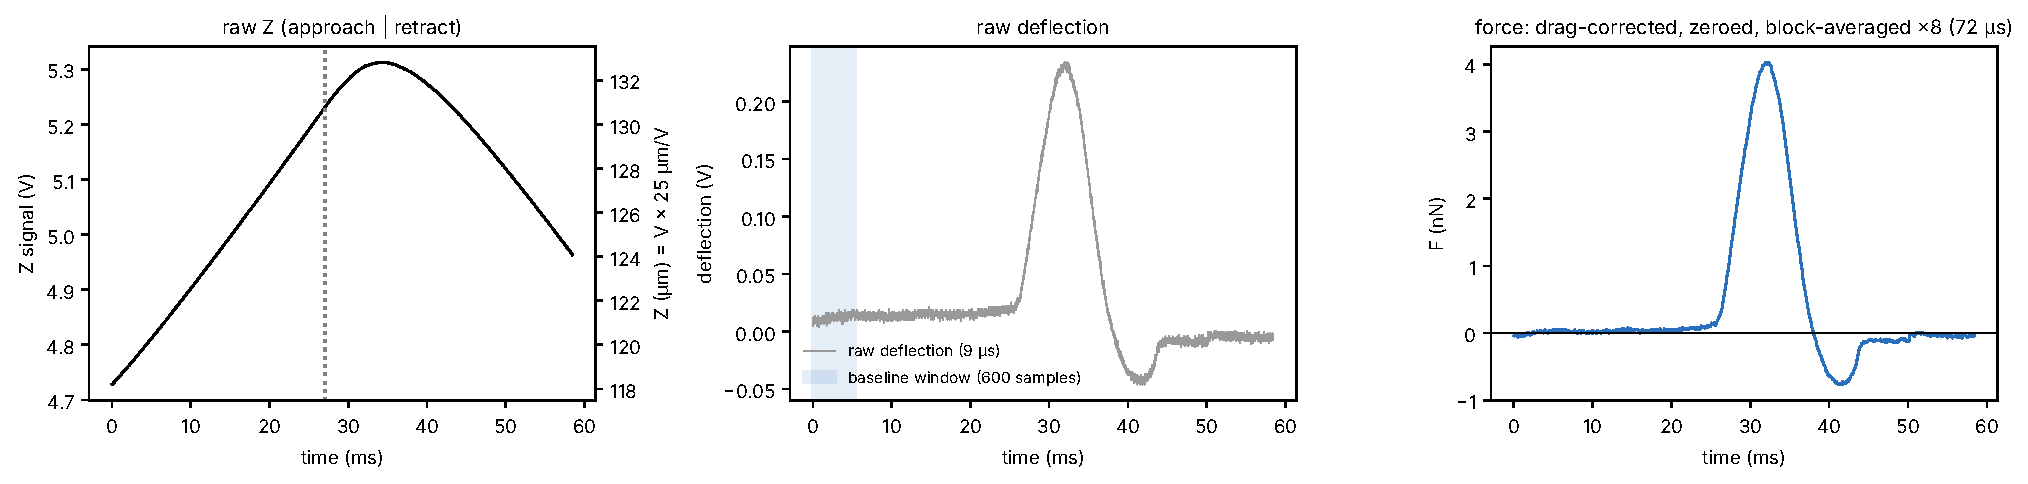
\includegraphics[width=\textwidth]{fig/raw_to_force.pdf}
\small
\begin{columns}[T]
\begin{column}{0.5\textwidth}
\begin{itemize}
\item One \texttt{.lvm} per pixel, one column: approach deflection (\texttt{num\_app} = 3000), retract deflection (3500), approach $Z$, retract $Z$ [V].
\item Sample interval $\Delta t$ = \texttt{loop\_time} = \SI{9}{\micro\second}.
\end{itemize}
\end{column}
\begin{column}{0.48\textwidth}
\begin{itemize}
\item $Z=\text{V}\times\SI{25}{\micro\metre\per\volt}$; deflection $d=\text{V}\times\text{InvOLS}$ (\SI{200}{\nano\metre\per\volt}).
\item $F=k\,d$, $k=\SI{0.09}{\newton\per\metre}=\SI{90}{\nano\newton\per\micro\metre}$.
\end{itemize}
\end{column}
\end{columns}
\end{frame}

\begin{frame}{Hydrodynamic drag correction}
\begin{columns}[T]
\begin{column}{0.55\textwidth}
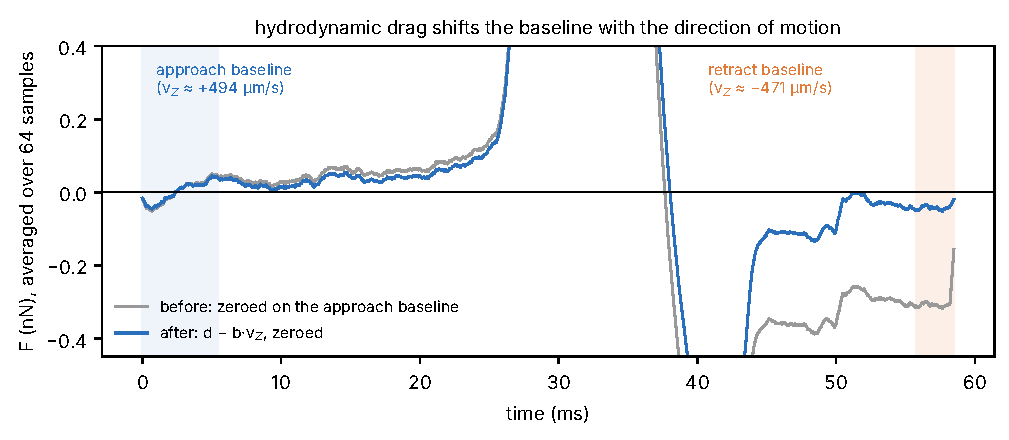
\includegraphics[width=\textwidth]{fig/drag.pdf}
\end{column}
\begin{column}{0.43\textwidth}\small
Moving through liquid adds a force proportional to the speed, $F_\text{drag}=-b\,v_Z$, which shifts the baseline in opposite directions on approach and retract.\\[3pt]
\textbf{Estimate} (300 curves spread over the map):
\[b=\med\frac{\med d_\text{app,base}-\med d_\text{ret,end}}{\med v_\text{app,base}-\med v_\text{ret,end}}\]
with $v_Z$ = derivative of the Savitzky--Golay smoothed $Z$ (window \SI{2.7}{\milli\second}, 3rd order).\\[3pt]
\textbf{Correction}: $d\leftarrow d-b\,v_Z(t)$ at every sample.\\[3pt]
Here: $v_\text{app}=\SI{494}{\micro\metre\per\second}$, $v_\text{ret}=\SI{471}{\micro\metre\per\second}$, $b=\SI{0.30}{\pico\newton\second\per\micro\metre}$. That is \SI{0.15}{\nano\newton} during the approach, about 3\,\% of the peak force.
\end{column}
\end{columns}
\end{frame}

\begin{frame}{Baseline, noise, block averaging}
\small
\begin{itemize}
\item \textbf{Force zero}: the median of the first 600 samples of the approach (\SI{5.4}{\milli\second}, probe far from the sample) is subtracted.
\item \textbf{Noise}: $\sigma=\mathrm{SD}(\text{first 600 samples})/\sqrt{8}$, i.e.\ the noise of a block-averaged point. Used for the contact threshold, and for the adhesion thresholds.
\item \textbf{Block averaging} by 8: \SI{9}{\micro\second}$\to$\SI{72}{\micro\second} per point, 6500 $\to$ 812 points per curve. This makes the fit 8$\times$ faster and cuts the noise by $\sqrt8$. The contact lasts $\approx\SI{11}{\milli\second}$ ($\approx150$ points), so time resolution is not lost.
\item The model is evaluated on exactly these points (uniform time grid).
\end{itemize}
\textbf{Config}:
\begin{itemize}
\item \texttt{[preprocessing] baseline\_samples} = auto ($\min(600,\ \texttt{num\_app}/3)$);
\item \texttt{block\_average} = auto ($\approx800$ points per curve);
\item \texttt{z\_smoothing\_ms} = 2.7;
\item \texttt{drag\_correction} = true.
\end{itemize}
\end{frame}

\begin{frame}{Tip position, contact point and indentation}
\begin{columns}[T]
\begin{column}{0.42\textwidth}
\centering
\resizebox{\linewidth}{!}{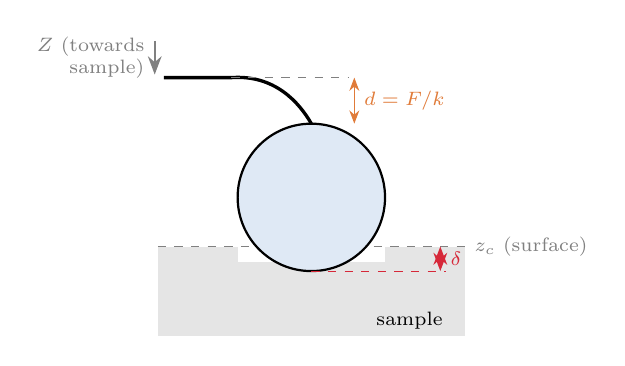
\begin{tikzpicture}[scale=0.78,>=Stealth]
 \fill[gray!20] (-0.4,0) rectangle (4.6,-1.2); \node[font=\scriptsize] at (3.7,-0.95) {sample};
 \draw[dashed,gray] (-0.4,0.25) -- (4.6,0.25) node[right,font=\scriptsize]{$z_c$ (surface)};
 \fill[gray!20] (0.9,0.0) -- (0.9,0.25) -- (-0.4,0.25) -- (-0.4,0) -- cycle;
 \fill[gray!20] (3.3,0.0) -- (3.3,0.25) -- (4.6,0.25) -- (4.6,0) -- cycle;
 \draw[thick,fill=cBlue!15] (2.1,1.05) circle (1.2);
 \draw[<->,cRed,thick] (4.2,0.25) -- (4.2,-0.15) node[midway,right,font=\scriptsize]{$\delta$};
 \draw[dashed,cRed] (2.1,-0.15) -- (4.3,-0.15);
 \draw[very thick] (-0.3,3.0) -- (0.8,3.0) .. controls (1.5,3.05) and (1.9,2.6) .. (2.1,2.25);
 \draw[dashed,gray] (0.8,3.0) -- (2.7,3.0);
 \draw[<->,cOrange] (2.8,3.0) -- (2.8,2.25) node[midway,right,font=\scriptsize]{$d=F/k$};
 \draw[->,thick,gray] (-0.45,3.6) -- (-0.45,3.05) node[midway,left,font=\scriptsize,align=right]{$Z$ (towards\\sample)};
\end{tikzpicture}}
\end{column}
\begin{column}{0.56\textwidth}\small
\begin{itemize}
\item $Z$ = stage extension towards the sample. The cantilever bends up by $d=F/k$ when pushing, so the probe advances less than the stage:
\[s(t)=Z(t)-d(t)\quad\text{(tip position)}\]
\item Contact point $z_c$ = tip position where the probe touches the surface. Indentation:
\[\delta(t)=\max\bigl(s(t)-z_c,\ 0\bigr)\]
\item $z_c$ is not read off the curve; it is a \textbf{fit parameter}. Its start value comes from a threshold (next slides).
\item Topography: $Z_c$ = stage position at which the tip reaches $z_c$; height $=\max(Z_c)-Z_c$ over the map.
\end{itemize}
Curve \#103: $F_\text{max}=\SI{4.03}{\nano\newton}\Rightarrow d=\SI{45}{\nano\metre}$, $\delta_\text{max}=\SI{2.15}{\micro\metre}$.
\end{column}
\end{columns}
\end{frame}

% ===========================================================================
\section{Contact mechanics}

\begin{frame}{Elastic indentation law $\varphi(\delta)$}
\begin{columns}[T]
\begin{column}{0.48\textwidth}
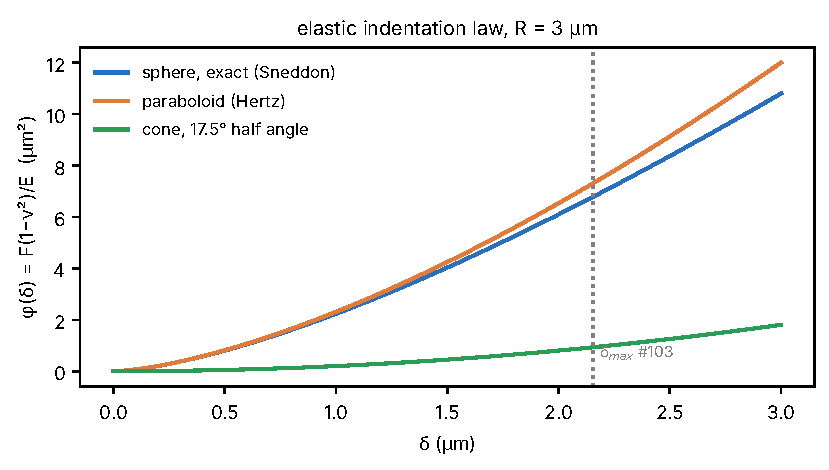
\includegraphics[width=\textwidth]{fig/contactlaws.pdf}
\end{column}
\begin{column}{0.5\textwidth}\small
For an elastic half-space, $F=\dfrac{E}{1-\nu^2}\,\varphi(\delta)$:\\[3pt]
\textbf{Sphere, exact} (Sneddon), parametric in $u=a/R$ ($a$ = contact radius):
\[\frac{\delta}{R}=\frac u2\ln\frac{1+u}{1-u},\quad \frac{\varphi}{R^2}=\frac{u^2+1}{2}\ln\frac{1+u}{1-u}-u\]
tabulated for $0\le u<1$ and interpolated.\\[3pt]
\textbf{Paraboloid} (Hertz, $\delta\ll R$): $\varphi=\tfrac43\sqrt R\,\delta^{3/2}$\\[3pt]
\textbf{Cone} (half angle $\theta$): $\varphi=\tfrac2\pi\tan\theta\,\delta^2$\\[4pt]
Here $\delta_\text{max}\approx\SI{1.7}{\micro\metre}$ (median) is not small against $R=\SI{3}{\micro\metre}$, so the exact sphere is used. At $\delta=\SI{2.15}{\micro\metre}$ it gives 7\,\% less force than Hertz.\\[3pt]
\textbf{Config}: \texttt{[probe] geometry, radius\_um, half\_angle\_deg, poisson\_ratio}
\end{column}
\end{columns}
\end{frame}

% ===========================================================================
\section{Viscoelasticity}

\begin{frame}{Power-law relaxation: what $E_1$ and $\alpha$ mean}
\begin{columns}[T]
\begin{column}{0.48\textwidth}
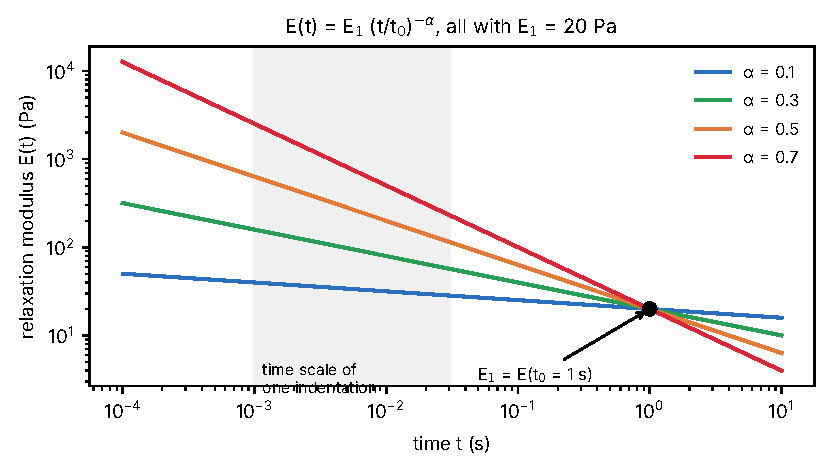
\includegraphics[width=\textwidth]{fig/powerlaw.pdf}
\end{column}
\begin{column}{0.5\textwidth}\small
\[E(t)=E_1\,(t/t_0)^{-\alpha}\]
\begin{itemize}
\item $\bm\alpha$: how fast stress relaxes, and the ratio of loss to storage, $\tan\delta_\text{loss}=\tan(\pi\alpha/2)$:
 \begin{itemize}
 \item $\alpha=0$: elastic solid (no relaxation);
 \item $\alpha=1$: Newtonian liquid;
 \item cells typically 0.1--0.5. Here the median is 0.50 (IQR 0.48--0.53).
 \end{itemize}
\item $\bm{E_1}$: the modulus at $t=t_0=\SI{1}{\second}$. This is a convention of the scale, not a measured time.
\item One indentation lasts $\approx\SI{11}{\milli\second}$ (\#103: loading \SI{7.8}{\milli\second}). $E_1$ is therefore an \textbf{extrapolation over two decades} in time. The moduli at the time scale of the measurement, $E(\SI{2}{\milli\second})$ and $E(\SI{10}{\milli\second})$, are stored as well (\texttt{[fit] tref\_s}).
\item Changing $t_0$ changes only the reference value: $E(t)$ and $\alpha$ stay the same.
\end{itemize}
\end{column}
\end{columns}
\end{frame}

\begin{frame}{Loading and unloading: Lee--Radok and Ting}
\begin{columns}[T]
\begin{column}{0.6\textwidth}
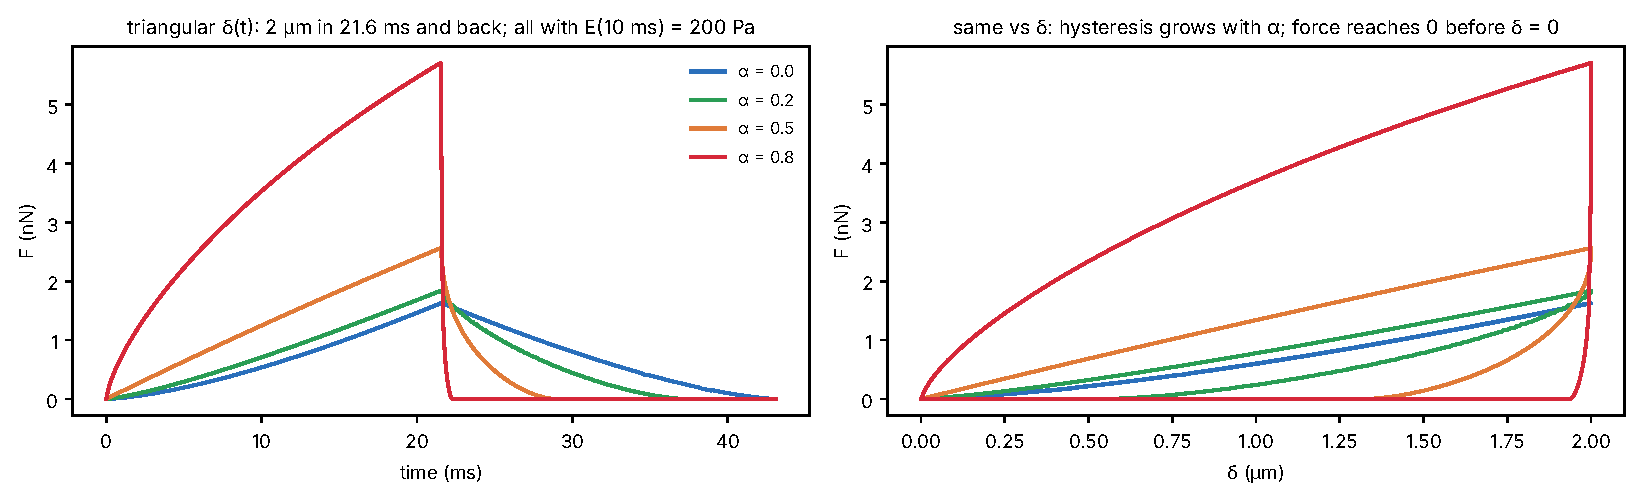
\includegraphics[width=\textwidth]{fig/alpha_effect.pdf}\\
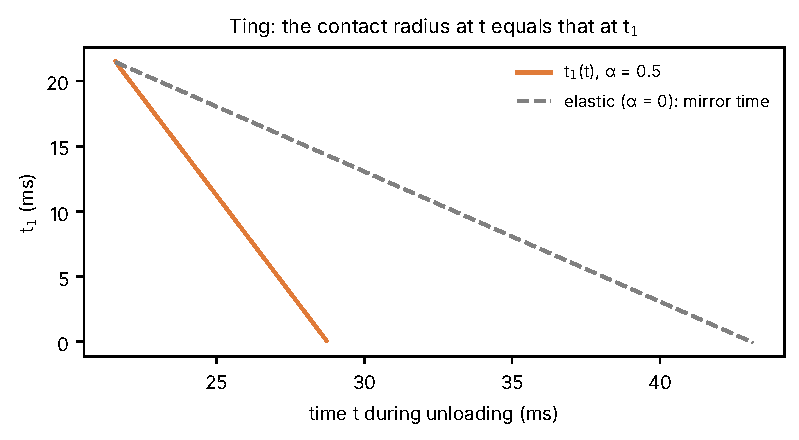
\includegraphics[width=0.62\textwidth]{fig/t1.pdf}
\end{column}
\begin{column}{0.38\textwidth}\footnotesize
\textbf{Loading} ($t\le t_m$, contact area grows): the force is the superposition of all earlier increments $d\varphi$, each relaxing with $E(t-\tau)$ (Lee--Radok).\\[3pt]
\textbf{Unloading} ($t>t_m$): the contact area shrinks. Lee--Radok would give tensile (negative) contact pressures, which is unphysical. Ting's solution: the contact radius at time $t$ equals the one at an earlier time $t_1(t)\le t_m$, defined by
\[\int_{t_1}^{t}E(t-\tau)\,\dot\delta(\tau)\,d\tau=0,\]
and the force uses the history only up to $t_1$.\\[3pt]
For $\alpha=0$, $t_1$ is the mirror time and the curve retraces itself. With larger $\alpha$ the hysteresis grows, and the force reaches 0 before $\delta=0$: the probe leaves the slowly recovering surface.
\end{column}
\end{columns}
\end{frame}

\begin{frame}{Discretisation (as implemented)}
\small
Uniform grid $t_n=n\,\Delta t$ ($\Delta t=\SI{72}{\micro\second}$), contact at the first sample with $s>z_c$, increments $\Delta\varphi_j=\varphi(\delta_{j+1})-\varphi(\delta_j)$, $\Delta\delta_j=\delta_{j+1}-\delta_j$.\\[4pt]
\textbf{Kernel} = mean of $E(\tau)/E_1$ over each time step. This is exact for the power law and avoids the singularity at $\tau=0$:
\[w_m=\frac1{\Delta t}\int_{(m-1)\Delta t}^{m\Delta t}\Bigl(\frac{\tau}{t_0}\Bigr)^{-\alpha}d\tau=\frac{t_0^{\alpha}\,\Delta t^{-\alpha}}{1-\alpha}\bigl(m^{1-\alpha}-(m-1)^{1-\alpha}\bigr)\]
\textbf{Loading} ($n\le m^*$, $m^*$ = index of $\max\delta$):
\[g_n=\sum_{j=0}^{n-1}w_{n-j}\,\Delta\varphi_j\qquad\text{(a convolution)}\]
\textbf{Unloading} ($n>m^*$):
\begin{itemize}
\item $R_n(j)=\sum_{j'=j}^{n-1}w_{n-j'}\,\Delta\delta_{j'}$;
\item $j_1$ = the last $j\le m^*$ with $R_n(j)\ge0$; the fraction $f$ between $j_1$ and $j_1+1$ is interpolated linearly in $R$;
\item $g_n=\max\Bigl(0,\ \sum_{j<j_1}w_{n-j}\Delta\varphi_j+(1-f)\,w_{n-j_1}\Delta\varphi_{j_1}\Bigr)$.
\end{itemize}
\textbf{Model force}: $F^\text{model}_n=E_1\,g_n/(1-\nu^2)$. $E_1$ is a pure scale factor.
\end{frame}

\begin{frame}{The fit}
\small
\textbf{Window}: from the first sample of the curve (including the non-contact baseline, where the model is 0) to the first sample after the peak where the smoothed force is $<0$. Approach and retract are fitted together, in time.\\[4pt]
\textbf{$E_1$ in closed form}: for given $(\alpha,z_c)$ the model is linear in $E_1$:
\[E_1^*(\alpha,z_c)=\max\Bigl(0,\ \frac{\mathbf g^\top\mathbf F}{\mathbf g^\top\mathbf g}\Bigr)\qquad(\mathbf g\text{ including }1/(1-\nu^2))\]
\textbf{Nonlinear part} (variable projection): minimise
\[\tfrac12\sum_n\bigl(E_1^*\,g_n(\alpha,z_c)-F_n\bigr)^2\]
over $(\alpha, z_c)$ only, by trust-region least squares (\texttt{scipy least\_squares}, TRF) with bounds
\[0\le\alpha\le0.95,\qquad s_{c,0}-\SI{4}{\micro\metre}\le z_c\le s_{c,0}+\SI{1.5}{\micro\metre}.\]
Two starts are tried ($\alpha=0.3$; $z_c=s_{c,0}$ and $s_{c,0}-\SI{0.4}{\micro\metre}$) and the lower cost is kept.\\[4pt]
\textbf{Start contact} $s_{c,0}$: the last point before the peak where the force, smoothed over 9 points, is below $\max(4\sigma,\ 0.03\,F_\text{max})$.\\[4pt]
\textbf{Goodness}: $R^2=1-\sum(F^\text{model}-F)^2/\sum(F-\bar F)^2$, over the window from 10 points before $s_{c,0}$.
\end{frame}

% ===========================================================================
\section{Worked example and parameter effects}

\begin{frame}{Example: curve \#103}
\centering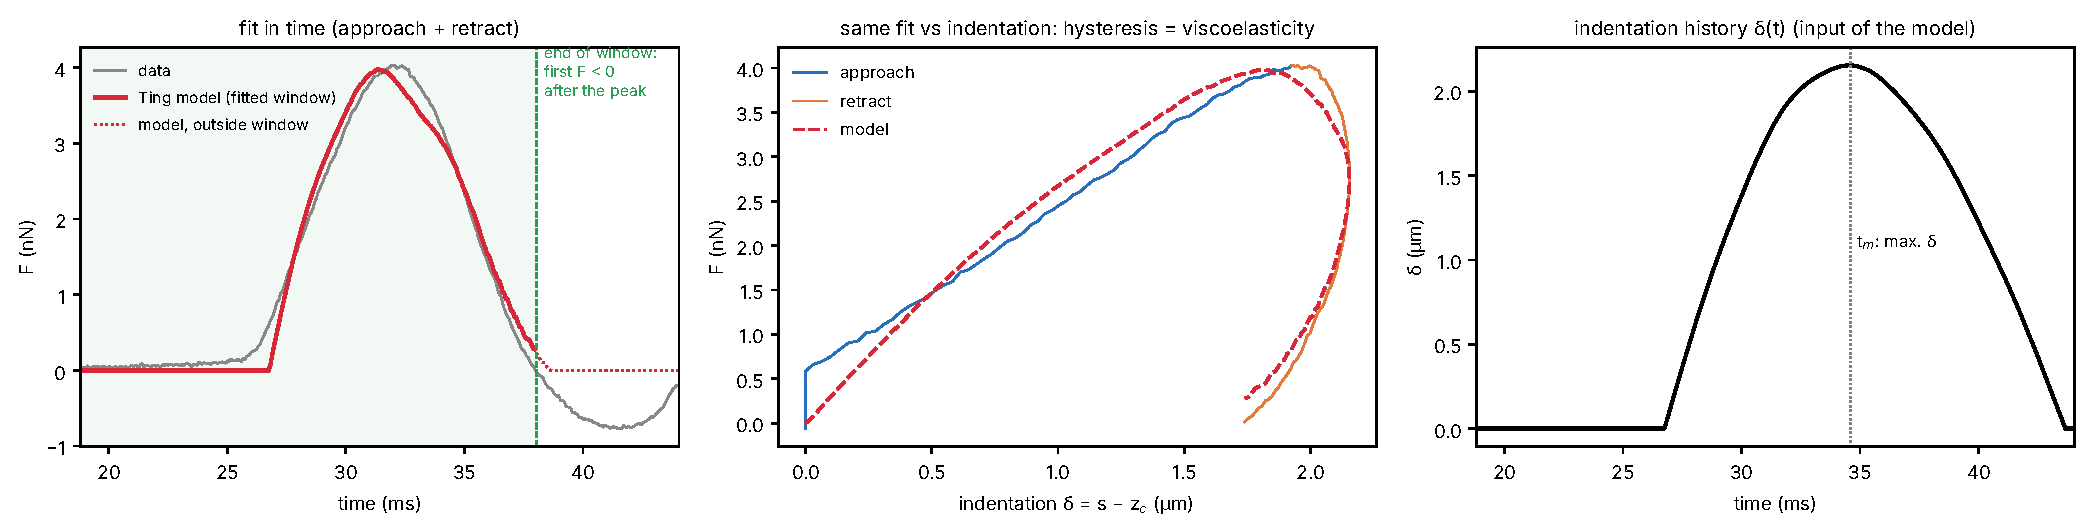
\includegraphics[width=\textwidth]{fig/fit103.pdf}
\small
\begin{columns}[T]
\begin{column}{0.5\textwidth}
\textbf{Vertical fit}:
\begin{itemize}
\item $E_1=\SI{17.7}{\pascal}$, $\alpha=0.508$;
\item $E(\SI{2}{\milli\second})=\SI{418}{\pascal}$, $E(\SI{10}{\milli\second})=\SI{184}{\pascal}$;
\item $\delta_\text{max}=\SI{2.15}{\micro\metre}$, $F_\text{max}=\SI{4.03}{\nano\newton}$, $R^2=0.975$.
\end{itemize}
\end{column}
\begin{column}{0.48\textwidth}
The retract part (orange) lies below the approach: the sample has relaxed. The model reproduces this hysteresis with a single $\alpha$.
\end{column}
\end{columns}
\end{frame}

\begin{frame}{The contact point in practice}
\begin{columns}[T]
\begin{column}{0.52\textwidth}
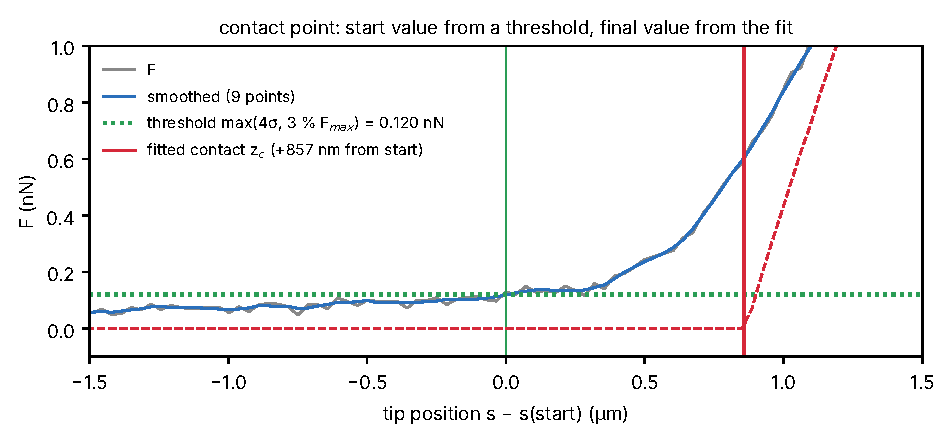
\includegraphics[width=\textwidth]{fig/contact.pdf}
\end{column}
\begin{column}{0.46\textwidth}\small
\begin{itemize}
\item The threshold gives only the start value. The fit then places $z_c$ where the curve shape is best described by the model.
\item In this data the fitted contact lies \textbf{\SI{0.67}{\micro\metre} beyond the threshold point} (median over 2775 curves; 5--95\,\%: 0.39--1.52\um). There the measured force is already \SI{0.67}{\nano\newton} (median, $\approx13\,\%$ of $F_\text{max}$).
\item So the curves begin with a soft ``toe'' that the model of a homogeneous half-space does not describe (possible causes: a pericellular coat, microvilli, an uneven contact under the bead). $\delta$ is counted from where the bulk response starts.
\item Consequence: $E$ describes the bulk under the toe, and the toe itself is not quantified.
\end{itemize}
\end{column}
\end{columns}
\end{frame}

\begin{frame}{What each fitted parameter does to the curve}
\centering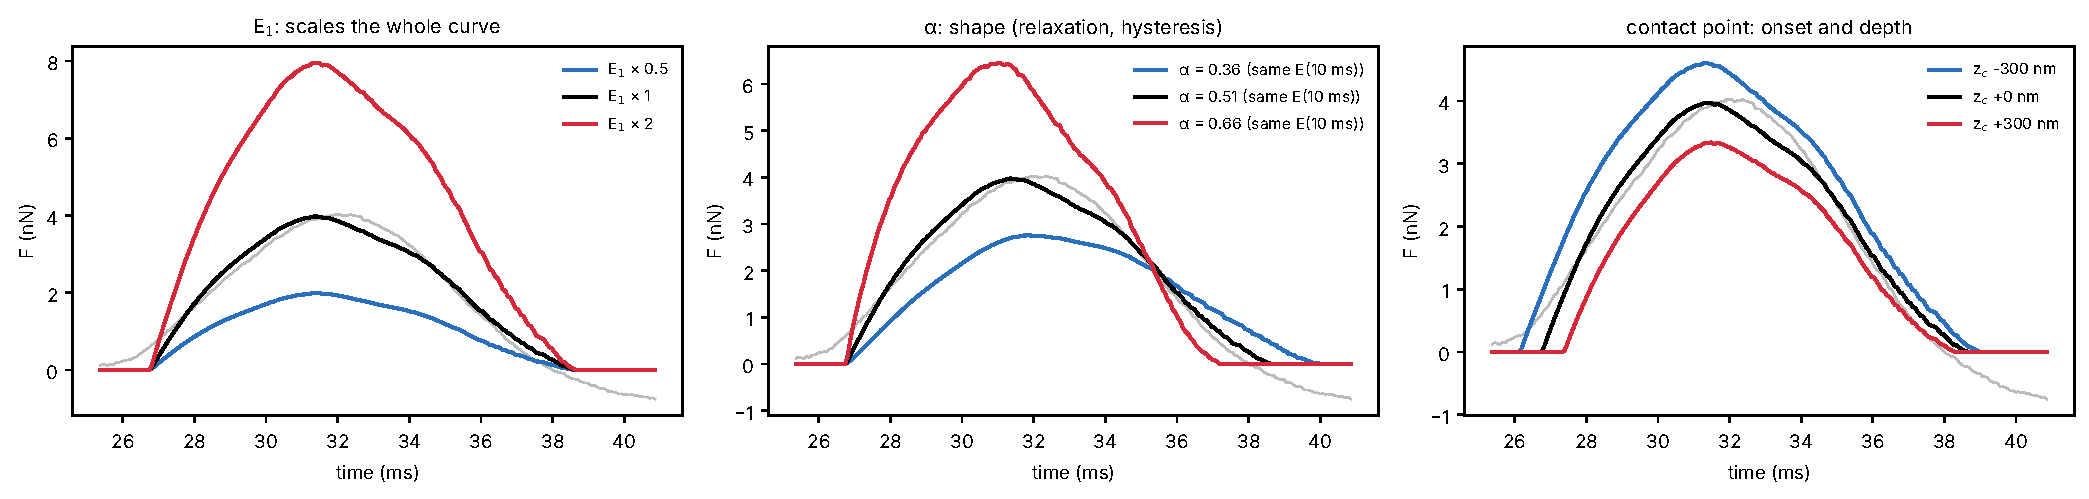
\includegraphics[width=\textwidth]{fig/param_effects.pdf}
\small
\begin{itemize}
\item $\bm{E_1}$ multiplies the whole model curve. It changes the amplitude, not the shape.
\item $\bm\alpha$ (here at the same $E(\SI{10}{\milli\second})$) changes the shape. A larger $\alpha$ gives a steeper rise during fast loading, more relaxation, a stronger drop on unloading and an earlier return to $F=0$.
\item $\bm{z_c}$ moves the onset, and with it the indentation depth. A later contact means less $\delta$, so a stiffer $E$ is needed for the same force.
\end{itemize}
\end{frame}

\begin{frame}{Are $E_1$ and $\alpha$ separable?}
\centering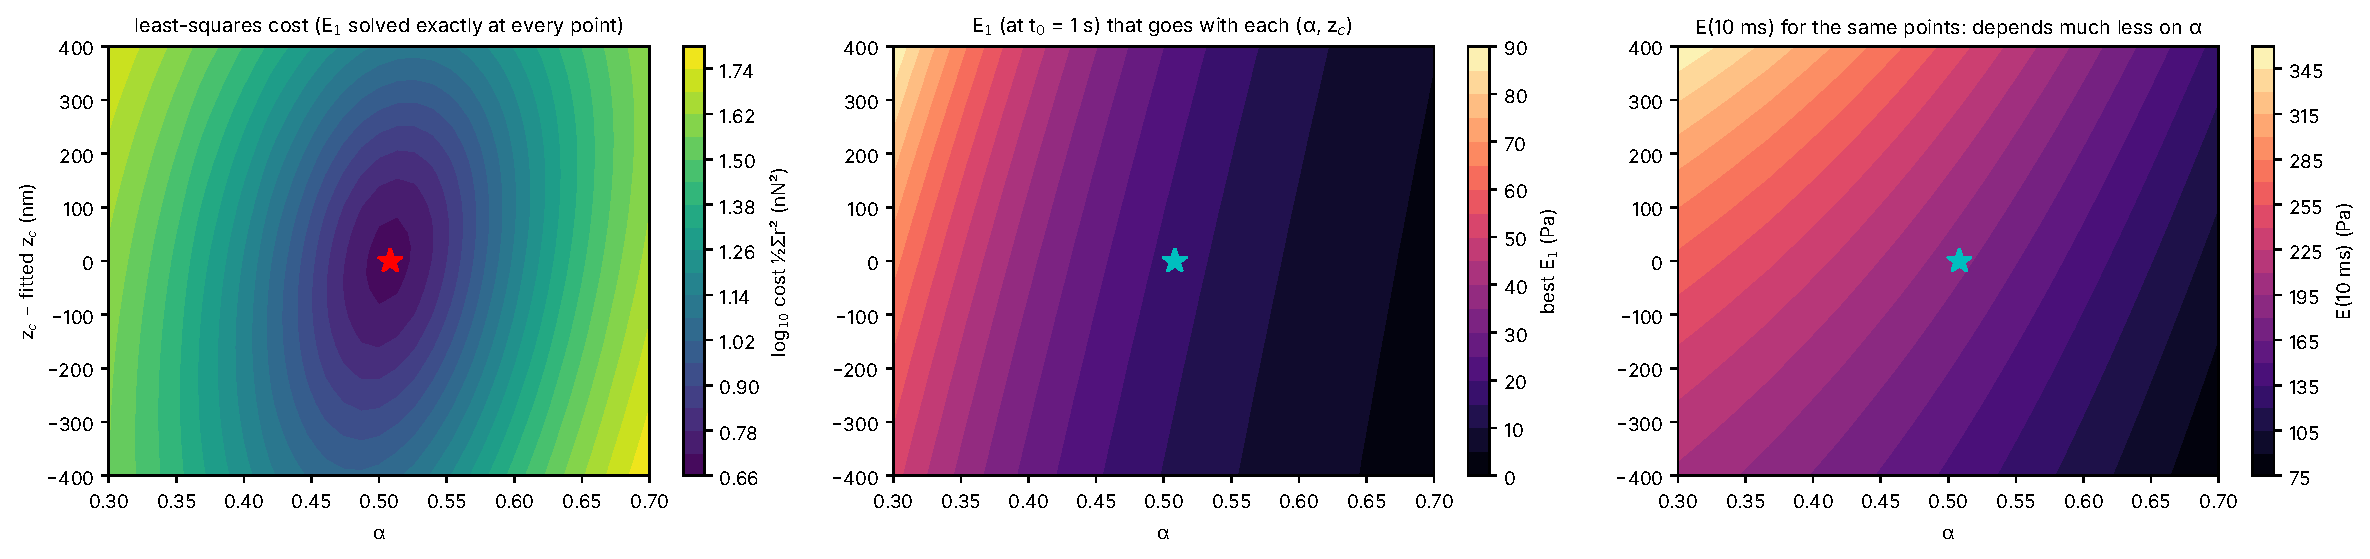
\includegraphics[width=\textwidth]{fig/landscape.pdf}
\small
\begin{columns}[T]
\begin{column}{0.5\textwidth}
\begin{itemize}
\item The cost has one well-defined minimum in $(\alpha,z_c)$ (left), so both are determined by a single curve.
\item But $E_1$ is strongly tied to $\alpha$ because it is extrapolated to \SI{1}{\second}. Along $\alpha=0.3\to0.7$ (at the fitted $z_c$), $E_1$ goes from 66.8 to \SI{3.9}{\pascal} (17$\times$), while $E(\SI{10}{\milli\second})$ goes from 266 to \SI{98}{\pascal} (2.7$\times$).
\end{itemize}
\end{column}
\begin{column}{0.48\textwidth}
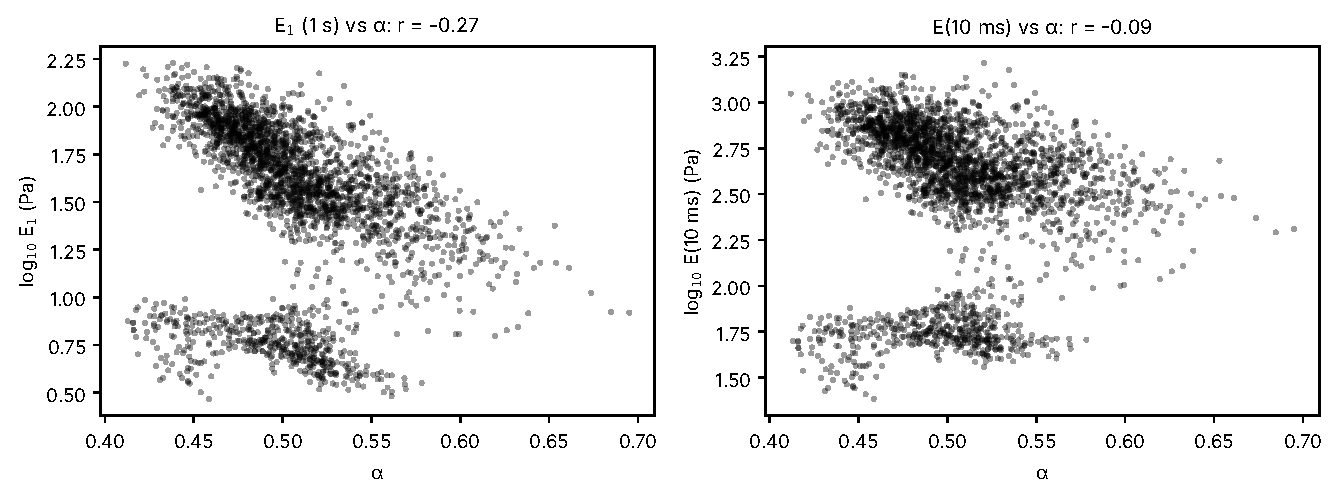
\includegraphics[width=\textwidth]{fig/coupling.pdf}\\
\scriptsize Over the map: correlation of $\log E_1$ with $\alpha$, $r=-0.27$; of $\log E(\SI{10}{\milli\second})$ with $\alpha$, $r=-0.09$.\\
\textbf{Use $E(2\text{ or }\SI{10}{\milli\second})$ to compare stiffness}, and $E_1$ only together with $\alpha$.
\end{column}
\end{columns}
\end{frame}

% ===========================================================================
\section{Surface-slope correction}

\begin{frame}{Surface-slope correction}
\begin{columns}[T]
\begin{column}{0.38\textwidth}
\centering
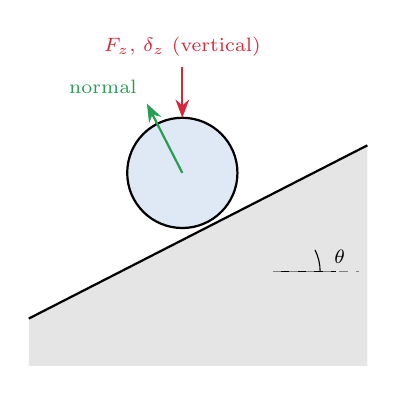
\begin{tikzpicture}[scale=1.0,>=Stealth]
 \fill[gray!20] (-0.5,-0.6) -- (3.8,1.6) -- (3.8,-1.2) -- (-0.5,-1.2) -- cycle;
 \draw[thick] (-0.5,-0.6) -- (3.8,1.6);
 \draw[thick,fill=cBlue!15] (1.45,1.25) circle (0.7);
 \draw[->,thick,cRed] (1.45,2.6) -- (1.45,1.95) node[pos=0,above,font=\scriptsize]{$F_z$, $\delta_z$ (vertical)};
 \draw[->,thick,cGreen] (1.45,1.25) -- ++(-0.45,0.88) node[above left,font=\scriptsize]{normal};
 \draw (2.6,0.0) -- (3.4,0.0); \draw (3.2,0.0) arc (0:27:0.6); \node[font=\scriptsize] at (3.45,0.18) {$\theta$};
 \draw[dashed,gray] (2.6,0.0) -- (3.7,0.0);
\end{tikzpicture}
\end{column}
\begin{column}{0.6\textwidth}\small
The probe moves vertically, but on a tilted surface it indents along the surface normal.
\begin{enumerate}
\item First, a vertical fit of all curves gives $z_c$, hence the topography.
\item Slope: $\theta=\arctan|\nabla(G_\sigma*\text{height})|$, with $\sigma$ = \texttt{slope\_smooth\_um} (auto: $\max(p_x,p_y,R/3)=\SI{1}{\micro\metre}$).
\item Refit every curve in the normal frame (contact force along the normal, no friction):
\[\delta_n=\delta_z\cos\theta,\qquad F_n=F_z/\cos\theta\qquad(\theta\le85^\circ)\]
\end{enumerate}
With $F\propto E\,\delta^{3/2}$ (Hertz), $E_n/E_z\approx\cos^{-5/2}\theta$:
\begin{itemize}
\item $\theta=\SI{19}{\degree}$ (\#103): 1.15 predicted, 1.14 fitted ($17.7\to\SI{20.2}{\pascal}$);
\item median slope \SI{38.8}{\degree}: 1.87 predicted, median ratio over the map 1.77.
\end{itemize}
Pixels with $\theta\ge\SI{60}{\degree}$ are flagged (the correction becomes unreliable). Both results are stored: \texttt{E1\_Pa} (normal) and \texttt{E1\_vertical\_Pa}.
\end{column}
\end{columns}
\end{frame}

% ===========================================================================
\section{Validity, outputs and maps}

\begin{frame}{Validity checks and the excluded map}
\small
\begin{tabularx}{\textwidth}{@{}l l X@{}}
\toprule
bit & criterion & meaning\\
\midrule
1 & $R^2\le$ \texttt{r2\_min} (0.9) & the model does not describe the curve\\
2 & slope $\ge$ \texttt{slope\_max\_deg} (60°) & normal-frame correction unreliable\\
4 & $\delta_\text{max}\ge$ \texttt{max\_delta\_over\_R} $\cdot R$ (2) & far beyond the validity of the contact model\\
8 & $\alpha\le0.001$, $\alpha\ge0.949$ or $E_1\le0$ & fit at a bound, so the parameter is not determined\\
16 & no fit & the curve could not be read or fitted\\
\bottomrule
\end{tabularx}\\[6pt]
\texttt{valid} = no bit set. In data\_213626, 2632 of 2775 curves (95\,\%) are valid and the median $R^2$ is 0.982.\\
\texttt{extract\_topo\_E.py} writes the bitmask to \texttt{excluded/}. With \texttt{no\_mask = true} the values stay in the maps and can be switched per reason in the viewer.
\end{frame}

\begin{frame}{Maps of data\_213626}
\begin{columns}[T]
\begin{column}{0.56\textwidth}
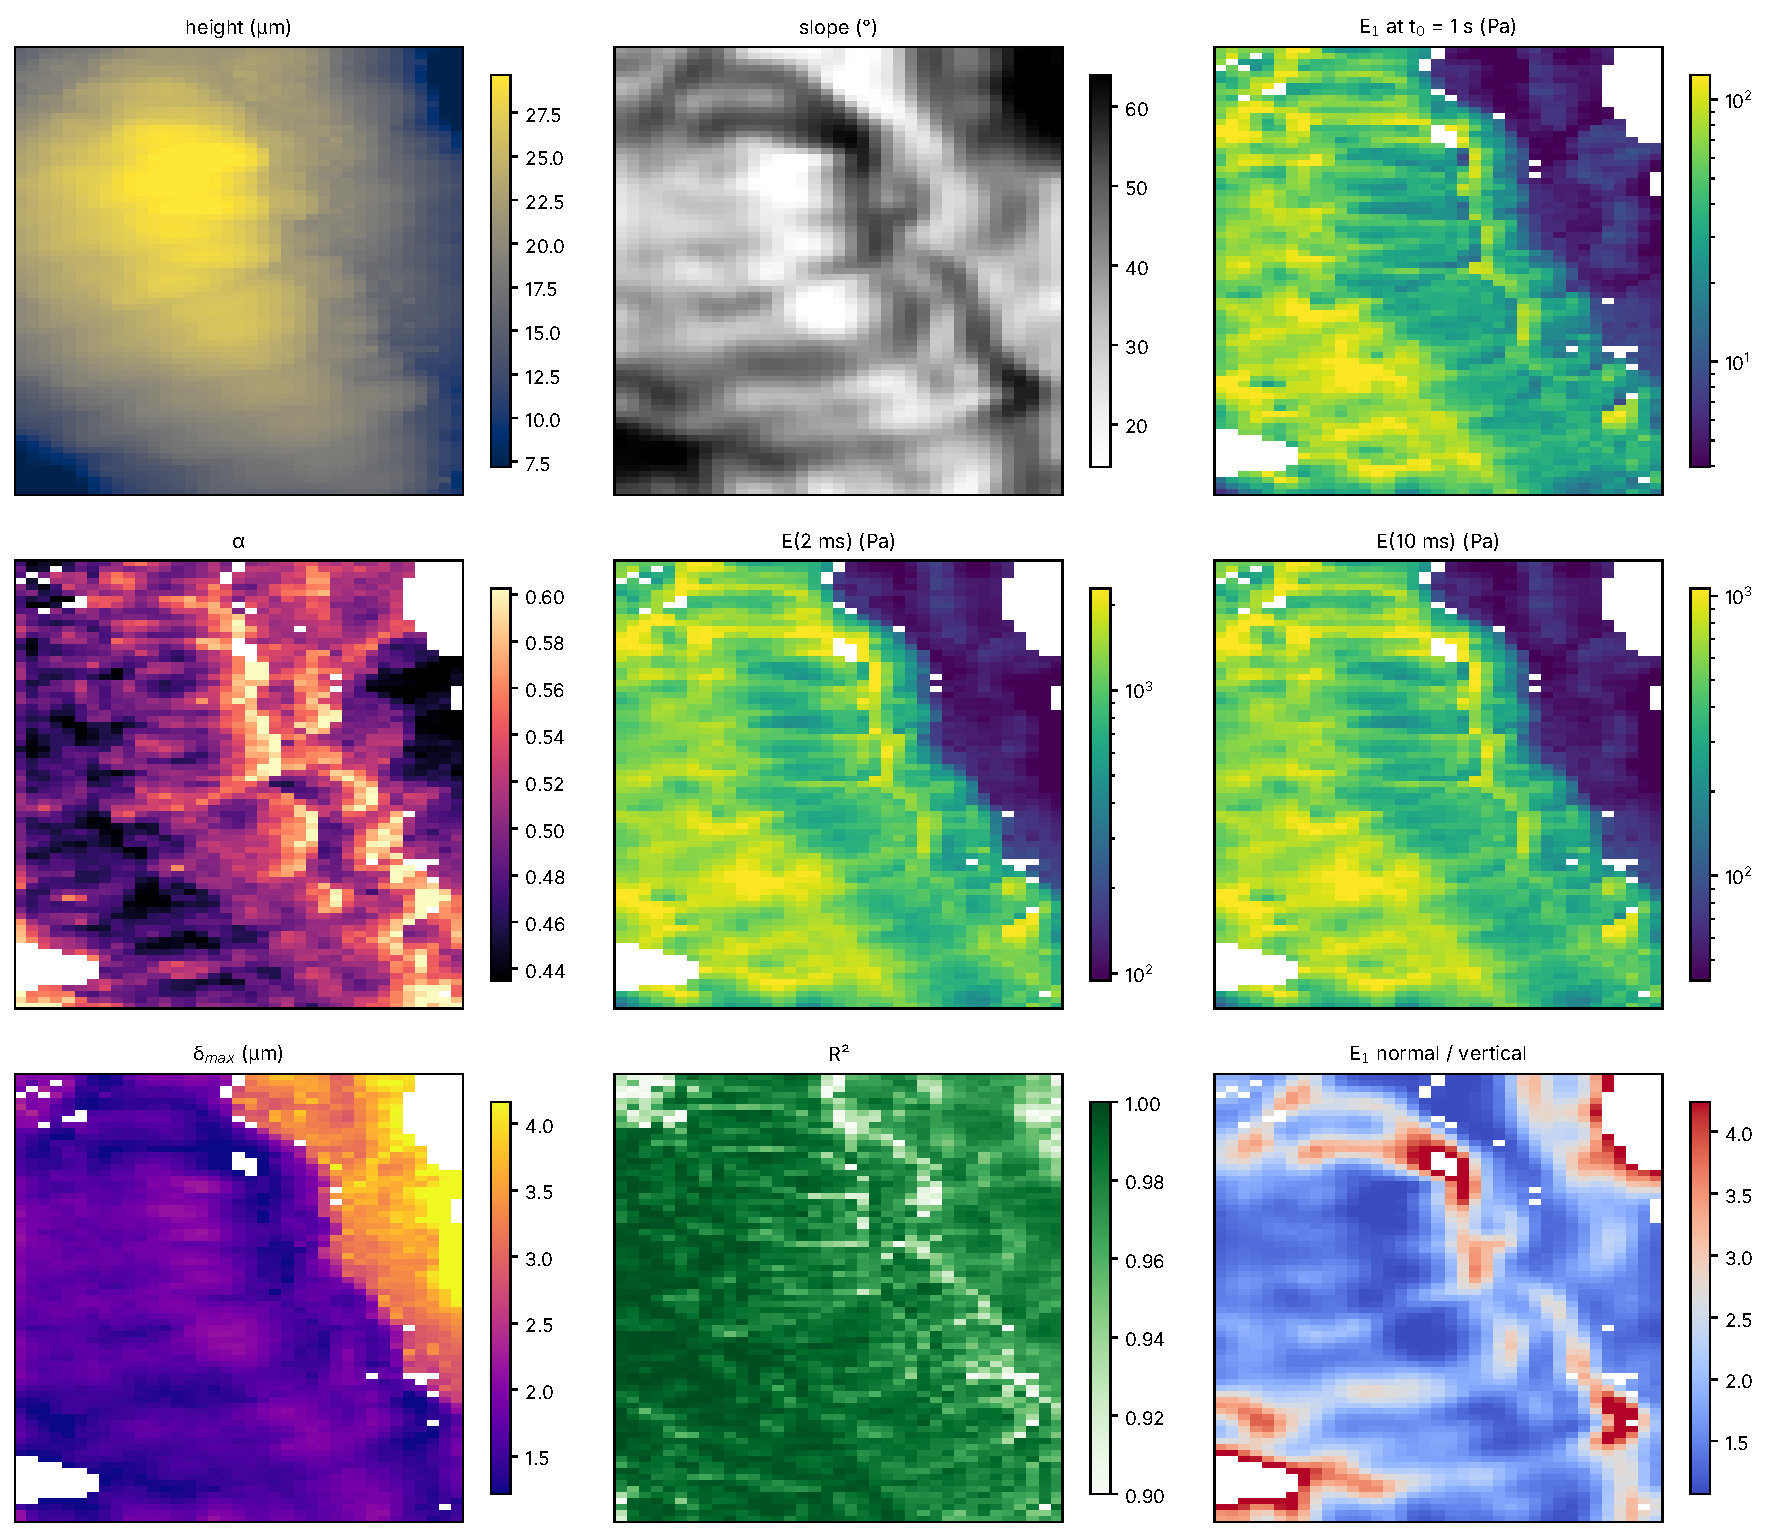
\includegraphics[width=\textwidth]{fig/maps.pdf}
\end{column}
\begin{column}{0.42\textwidth}\small
Medians of the valid pixels:
\begin{itemize}
\item $E_1=\SI{39}{\pascal}$ (IQR 21--69), $\alpha=0.50$ (0.48--0.53);
\item $E(\SI{2}{\milli\second})=\SI{999}{\pascal}$, $E(\SI{10}{\milli\second})=\SI{437}{\pascal}$;
\item $\delta_\text{max}=\SI{1.71}{\micro\metre}$, $F_\text{max}=\SI{5.1}{\nano\newton}$.
\end{itemize}
The steep flanks (high slope) carry the largest slope correction (last panel: up to $\times4$ near \SI{60}{\degree}). $E$ and $\alpha$ vary across the map with the slope pattern; horizontal streaks are scan-line effects.
\end{column}
\end{columns}
\end{frame}

\begin{frame}{Outputs per curve (in the \texttt{.npz})}
\scriptsize
\begin{tabularx}{\textwidth}{@{}l l X@{}}
\toprule
key & unit & content\\
\midrule
\texttt{E1\_Pa}, \texttt{alpha} & Pa, -- & normal-frame fit (slope-corrected)\\
\texttt{E1\_vertical\_Pa}, \texttt{alpha\_vertical} & Pa, -- & vertical fit\\
\texttt{E\_at\_2ms\_Pa}, \texttt{E\_at\_10ms\_Pa} & Pa & $E_1(t/t_0)^{-\alpha}$ at \texttt{tref\_s}\\
\texttt{delta\_max\_um}, \texttt{Fmax\_nN} & \si{\micro\metre}, nN & maximum indentation and force\\
\texttt{topo\_um}, \texttt{z\_contact\_um}, \texttt{slope\_deg} & \si{\micro\metre}, ° & topography from the contact point, slope\\
\texttt{R2}, \texttt{noise\_nN}, \texttt{valid} & & fit quality, baseline noise, validity\\
\texttt{cluster}, \texttt{cluster\_mean\_shape} & & k-means on peak-normalised curve shapes (PCA, 4 components)\\
\texttt{adh\_*} & & adhesion analysis of the retract curves (separate presentation)\\
\texttt{curves\_F\_nN}, \texttt{curves\_Fmodel\_nN}, \texttt{curves\_Z\_um}, \texttt{curves\_t\_s} & & all curves, block-averaged, with the model\\
\texttt{curve\_index\_map}, \texttt{x\_um}, \texttt{y\_um}, \texttt{pixel\_um} & & map geometry\\
\texttt{params\_json}, \texttt{config\_json} & & all parameters used, and the instrument's config.txt\\
\bottomrule
\end{tabularx}
\end{frame}

% ===========================================================================
\section{Parameters and limits}

\begin{frame}{Fit parameters in the config file and what they do}
\scriptsize
\begin{tabularx}{\textwidth}{@{}l l X@{}}
\toprule
key & default & effect\\
\midrule
\texttt{[afm] invols\_nm\_per\_V} & 200 & deflection scale. $F\propto$ InvOLS, and $d$ too, so $E$ scales almost $\propto$ InvOLS\\
\texttt{spring\_constant\_N\_m} & 0.09 & $F\propto k$ $\Rightarrow$ $E\propto k$ (nominal value; calibrate!)\\
\texttt{z\_sensitivity\_um\_per\_V} & 25 & scales $Z$, hence $\delta$ and the speeds\\
\texttt{[probe] geometry, radius\_um} & sphere, 3 & contact law. Hertz-like $E\propto R^{-1/2}$: $R=2.5$ instead of 3 gives $+9.5\,\%$\\
\texttt{poisson\_ratio} & 0.5 & $E\propto1-\nu^2$: $\nu=0.4$ gives $+12\,\%$\\
\texttt{[preprocessing] block\_average} & auto (8) & speed and noise vs.\ time resolution\\
\texttt{baseline\_samples} & auto (600) & force zero and noise $\sigma$; must lie before any contact\\
\texttt{drag\_correction}, \texttt{z\_smoothing\_ms} & true, 2.7 & baseline offset from viscous drag; smoothing of $Z$ for $v_Z$\\
\texttt{[fit] t0\_s} & 1 & reference time of $E_1$ only\\
\texttt{tref\_s} & 0.002, 0.01 & extra $E(t)$ maps (choose inside the contact time)\\
\texttt{slope\_correction}, \texttt{slope\_smooth\_um} & true, auto & normal-frame refit; smoothing of the height for the slope\\
\texttt{[quality] r2\_min, slope\_max\_deg, max\_delta\_over\_R} & 0.9, 60, 2 & validity bits 1, 2, 4\\
\bottomrule
\end{tabularx}\\[4pt]
Fixed in the code: the bounds of $\alpha$ $[0,0.95]$ and $z_c$ ($-4/+1.5$\um), the start values, the contact threshold $\max(4\sigma,3\%F_\text{max})$ and the end of the window ($F<0$).
\end{frame}

\begin{frame}{Limits}
\small
\begin{itemize}
\item \textbf{Calibration}: $k$ is nominal and $R$ is estimated from the topography. Both scale $E$ directly (previous slide); $\alpha$ is not affected.
\item \textbf{Contact model}: homogeneous, isotropic half-space, no friction, no adhesion inside the contact, sample much thicker than $\delta$. Cells are layered (cortex, cytoplasm), so $E$ is an effective modulus at $\delta\approx\SI{2}{\micro\metre}$.
\item \textbf{Toe region}: the first $\approx\SI{0.7}{\micro\metre}$ / \SI{0.7}{\nano\newton} of the contact is not described by the model and is effectively excluded from $\delta$.
\item \textbf{Power law} over the measured range only ($\approx$1--\SI{20}{\milli\second}): $E_1$ at \SI{1}{\second} is an extrapolation.
\item \textbf{Fit window} ends at $F=0$ on the retract. The adhesive part is analysed separately and not used for $E$ or $\alpha$.
\item \textbf{Slope correction} assumes the force acts along the normal. On steep flanks ($>\SI{60}{\degree}$), lateral forces and the probe side touching the sample make it unreliable.
\end{itemize}
\end{frame}

\begin{frame}{Summary}
\begin{itemize}
\item Force = drag-corrected, zeroed deflection $\times$ InvOLS $\times$ $k$. Indentation = tip position minus the fitted contact point.
\item The model is an exact Sneddon sphere with power-law relaxation. Lee--Radok is used for loading and Ting for unloading, discretised exactly on the \SI{72}{\micro\second} grid.
\item Per curve: $E_1$ is solved linearly; $\alpha$ and $z_c$ by bounded least squares on approach + retract (to $F=0$), in time.
\item The slope correction refits along the surface normal ($E_n/E_z\approx\cos^{-5/2}\theta$).
\item $\alpha$ and $E(\text{ms})$ are robust. $E_1$ at \SI{1}{\second} is an extrapolation and is tied to $\alpha$.
\item All parameters are in \texttt{afm\_pipeline.toml}, sections \texttt{[afm]}, \texttt{[probe]}, \texttt{[preprocessing]}, \texttt{[fit]} and \texttt{[quality]}.
\end{itemize}
\end{frame}

\end{document}
